\chapter{Architektur und Design Spezifikationen} \label{architecture-design-specification}

\section{Citations}
Im Buch \cite{starke}, Thesis \cite{riehle}, Paper \cite{treelayouter}, Online \cite{java-jigsaw}

\section{Glossary}
\gls{c4}, \gls{api}

\begin{figure}[H]
	\centering
	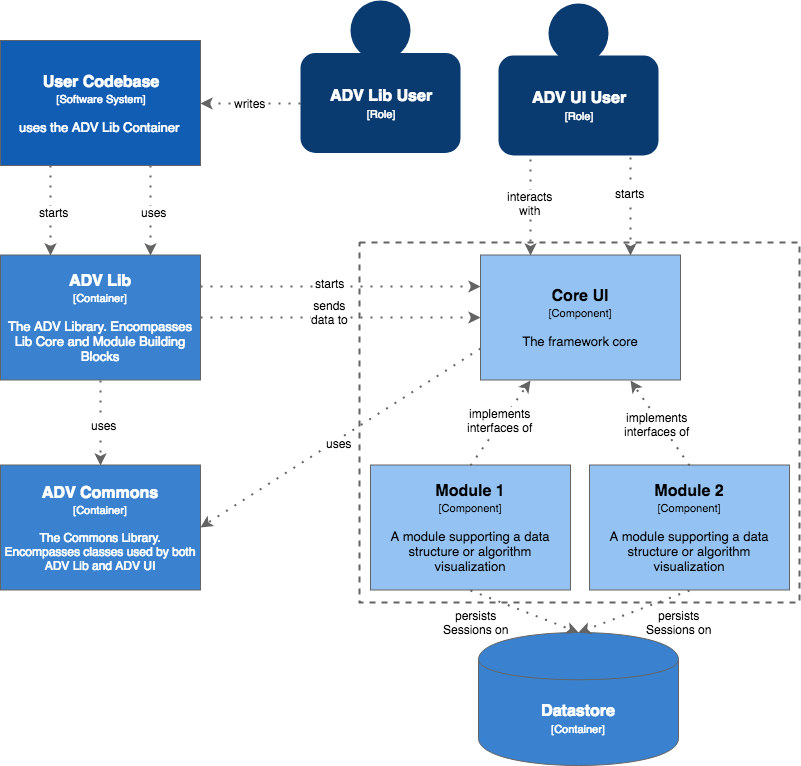
\includegraphics[width=0.7\textwidth]{attachments/c4/component-ui-diagram}
	\caption{Offizielle C4 Übersicht~\cite{c4}}
	\label{fig:c4-overview}
\end{figure}


\subsection{Code Listing}
\begin{lstlisting}[caption={Gradle}]
dependencies {
	compile 'ch.hsr.test:test:1.0'
}
\end{lstlisting}

Inline Code: \lstinline|java -jar test-<version>.jar|

\subsection{Image Explanation}
\begin{explanation}{attachments/c4/component-ui-diagram}
	Image Explanation
\end{explanation}

Circles with numbers to reference images: Click on button \circled{1}, \circled{2}, \circled{3a}


\subsection{Dir Tree}
\begin{table}[H]
	\centering
	\begin{tabularx}{\linewidth}{X X}
		\toprule 
		Projekt A & Projekt B \\
		\midrule
		\dirtree{%
			.1 A.
			.2 A1.
			.2 A2.
			.2 A3.
			.2 A4.
			.3 src.
			.4 main.
			.5 java.
			.6 C.
		}
		& 
		\dirtree{%
			.1 A.
			.2 A1.
			.2 A2.
			.2 A3.
			.2 A4.
			.3 src.
			.4 main.
			.5 java.
			.6 C.
		}
		\\
		\bottomrule 
	\end{tabularx} 
	\caption{Projekt Struktur} 
	\label{tbl:project-structure}
\end{table}


\subsection{Hints and Warnings}
\begin{hint}{Hint}{}
	See theoremsetup.tex
\end{hint}

\begin{warn}{Warning}{}
	See theoremsetup.tex
\end{warn}
